\chapter{Analysis Results and Systematic Errors}

\section{Fitting Method}

\section{Systematic Errors}

As with any experiment, \nova~is sensitive to a number of systematic effects. To combat this, \nova~was designed with two functionally identical detectors, so that Near Detector data can be used to constrain or correct the Far Detector prediction. Since many effects such as beam and cross section uncertainties affect the spectra at both detectors in a similar or the same way, this two detector technique leads to the reduction of these systematic errors. Other effects, such as Near Detector rock event contamination, require a data driven technique to quantify.

The general technique for analyzing systematic errors was to run the full extrapolation chain and generate a predicted spectrum with and without a systematic effect applied. Each given systematic effect was used to shift the MC simulation at one or both detectors as appropriate. The resulting difference between the shifted and nominal spectra was quantified as a systematic error.

The systematic effects analyzed included uncertainties arising from the beam, GENIE simulation, Birks-Chou light yield simulation, calibration, detector geometry simulation, light level effects, bias from the ND containment, ND rock event contamination, ND data/MC spectrum and hadronic energy differences, MC statistics, and overall normalization. The rest of this section discusses each of these effects in greater detail.

\subsection{Beam}

The \nova~MC simulation involves a fully detailed model of the NuMI beam process in an attempt to create the most realistic MC possible, but systematic errors can result from any mismatch between simulation and reality. The \nova~Beam Working Group performed studies to assess the effect that uncertainties in the simulation can have on the neutrino flux \cite{ref:TNBeam}. These studies included the effects of incorrectly modeling various parts of the beam transport and the effects of uncertainties in hadron production arising from fixed target experiments.

To quantify the systematic error caused by these beam uncertainties, a sample flux was generated using a systematic shift and compared to the nominal flux via a simple ratio. Results were generated separately for each neutrino flavor and for each detector. The ratios were used to modify the MC from the full simulation used as inputs to the extrapolated prediction. Finally, the shifted FD prediction was compared to the nominal prediction, with any differences being taken as the systematic error. At the end of this process, the individual errors were added in quadrature. Errors were calculated for the following systematics:
\begin{itemize}
  \item Beam position on target varied by $\pm 0.5\,mm$ in X
  \item Beam position on target varied by $\pm 0.5\,mm$ in Y
  \item Beam spot size varied by $\pm 0.2\,mm$ in both X and Y
  \item Target position varied by $+ 2\, mm$ in Z
  \item Horn current varied $\pm 1\,kA$
  \item Horn 1 position varied by $\pm 2\,mm$ in both X and Y
  \item Horn 2 position varied by $\pm 2\,mm$ in both X and Y
  \item Horn magnetic field changed from linear to exponential distribution
  \item Comparison between FLUKA and G4NuMI
  \item Comparison between FLUKA and NA49
\end{itemize}
\n Hadron production uncertainties were combined in quadrature before being provided as weights, so this is evaluated as single systematic error. The percentage difference due to each systematic is shown in Table \ref{tab:SystBeam}, and the full error envelopes for NC signal and background are shown in Fig.~\ref{fig:SystBeam}.
\begin{table}[h]
  \begin{center}
    \caption[Beam Systematic Errors]{The percentage difference between the shifted and nominal predictions for the number of FD events due to beam systematics.}
    \label{tab:SystBeam}
    \begin{tabular}{r c c}
      \hline\hline
      Systematic & NC Difference (\%) & Background Difference (\%) \\
      \hline
      Beam Position, X & & \\
      Beam Position, Y & & \\
      Beam Spot Size & & \\
      Target Position & & \\
      Horn Current & & \\
      Horn 1 Position & & \\
      Horn 2 Position & & \\
      Horn B Field & & \\
      Hadron Productions & & \\
      Combined & & \\
      \hline
    \end{tabular}
  \end{center}
\end{table}

\begin{figure}[h]
  \centering
  \begin{subfigure}{.48\textwidth}
    \centering
    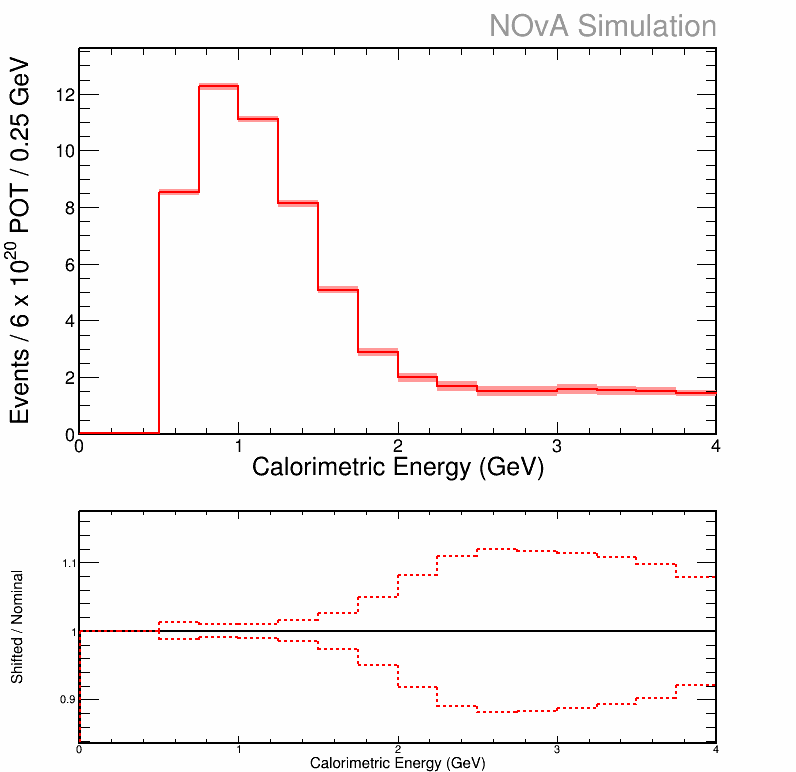
\includegraphics[width=1\linewidth]{figures/cNCEXBeamSysts.png}
  \end{subfigure}
  \begin{subfigure}{.48\textwidth}
    \centering
    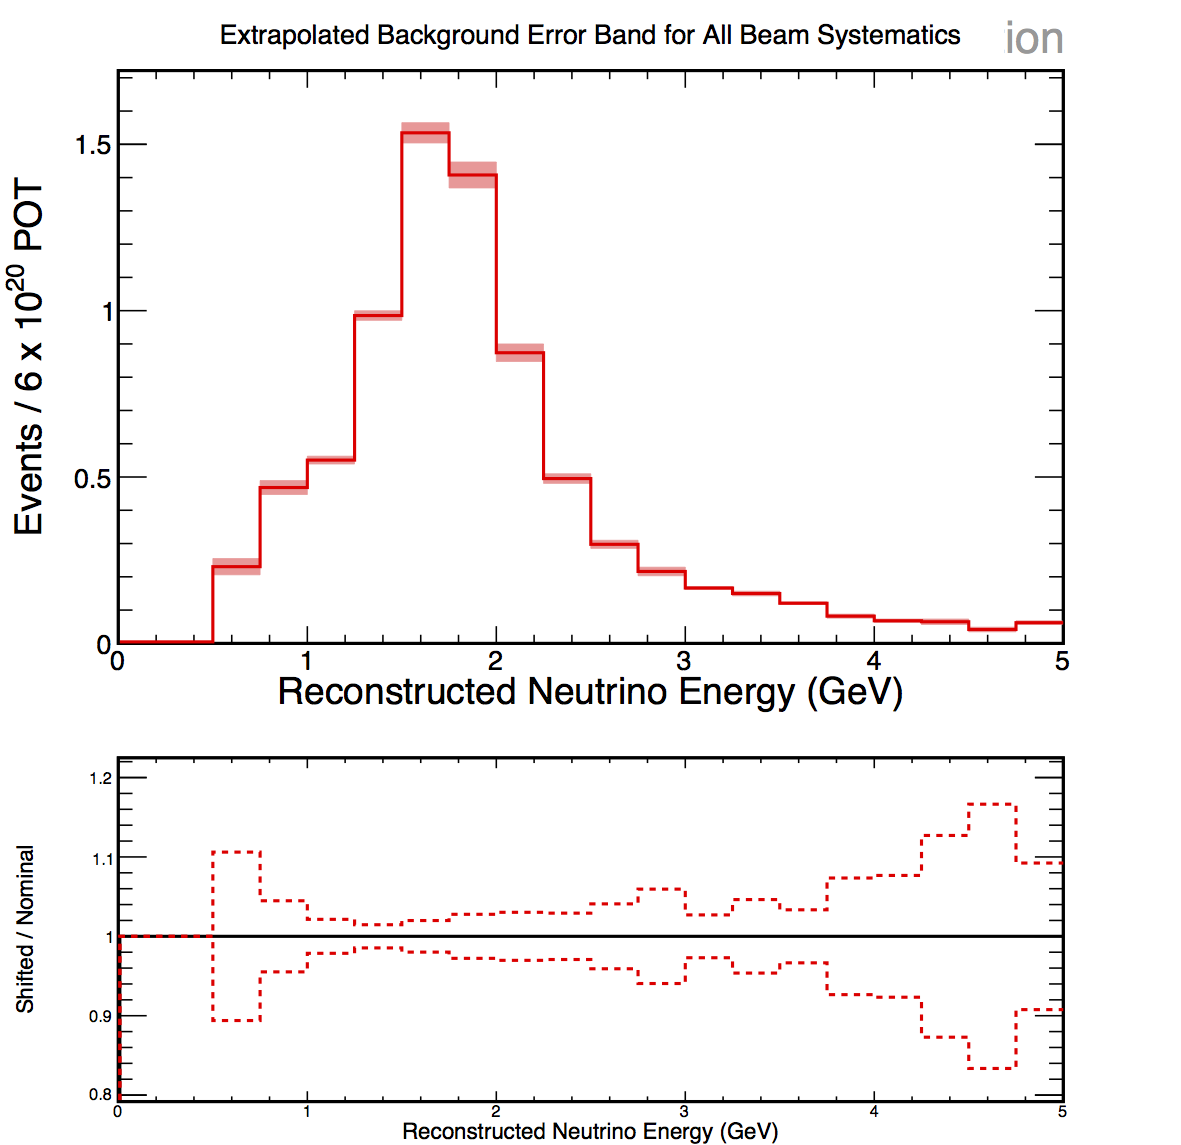
\includegraphics[width=1\linewidth]{figures/cBGEXBeamSysts.png}
  \end{subfigure}
  \caption[Beam Systematic Error Envelopes]{Systematic error envelope on the NC signal (left) and background (right) event spectra, after extrapolation. The envelope is calculated by adding in quadrature the larger of $\vert +1\sigma \vert$ and $\vert -1\sigma \vert$ for each individual systematic.}
  \label{fig:SystBeam}
\end{figure}

\subsection{Birks-Chou Light Yield Simulation}

The \nova~MC simulation employs the Birks-Chou Law to model the relationship between scintillator light yield, $LY$, and particle energy deposition rate, $\frac{dE}{dx}$ \cite{ref:BirksChou}. 
\beq
LY = A \frac{ \frac{dE}{dx} }{1 + k_B \frac{dE}{dx} + k_C \left( \frac{dE}{dx} \right)^2} 
\label{eq:BirksChou}
\eeq

\n This formula encapsulates the known light yield quenching that occurs for particles with a high energy deposition rate. The constants $k_B$ and $k_C$ are dependent on the scintillator material and had to be estimated for \nova~as no measurement existed for the particular material used in this experiment. A study was performed comparing the energy deposition at the end of proton tracks in the ND for both data and MC to find parameters that would generate agreement between the two \cite{ref:DanBirks}. The results of the study were $k_B = 0.04\unit{cm/MeV}$ and $k_C = -0.0005\unit{(cm/MeV)}^2$.

The systematic error based on the Birks-Chou light yield simulation was quantified by comparing the nominal FD prediction to predicted spectra using alternative Birks-Chou parameter constants. The values reported in the study from \cite{ref:DanBirks} were much larger than other typical measurements, so two MC samples were generated with more traditional values, one with $k_B = 0.01\unit{cm/MeV}$ called BirksB, the other with $k_B = 0.02\unit{cm/MeV}$ called BirksC, both with $k_C = 0$. Shifted FD event spectra were predicted by extrapolating the same set of ND data as the nominal prediction, but using the MC with alternative Birks-Chou model parameters. The error was taken as the percentage difference between the nominal and shifted predictions. Table \ref{tab:SystBirks} shows the percentage differences from both MC samples; fig.~\ref{fig:SystBirks} shows the shifted event spectra compared to nominal. Instead of combining the individual errors in quadrature, the shifted sample with the larger overall difference from the TODO model taken as the systematic error.
\begin{table}[h]
  \begin{center}
    \caption[Birks-Chou Systematic Errors]{The percentage difference between the shifted and nominal predictions for the number of FD events due to extrapolation using MC with alternative Birks-Chou model parameters.}
    \label{tab:SystBirks}
    \begin{tabular}{r c c}
      \hline\hline
      Model & NC Difference (\%) & Background Difference (\%) \\
      \hline
      BirksB & & \\
      BirksC & & \\
      \hline
    \end{tabular}
  \end{center}
\end{table}

\begin{figure}[h]
  \centering
  \begin{subfigure}{.48\textwidth}
    \centering
    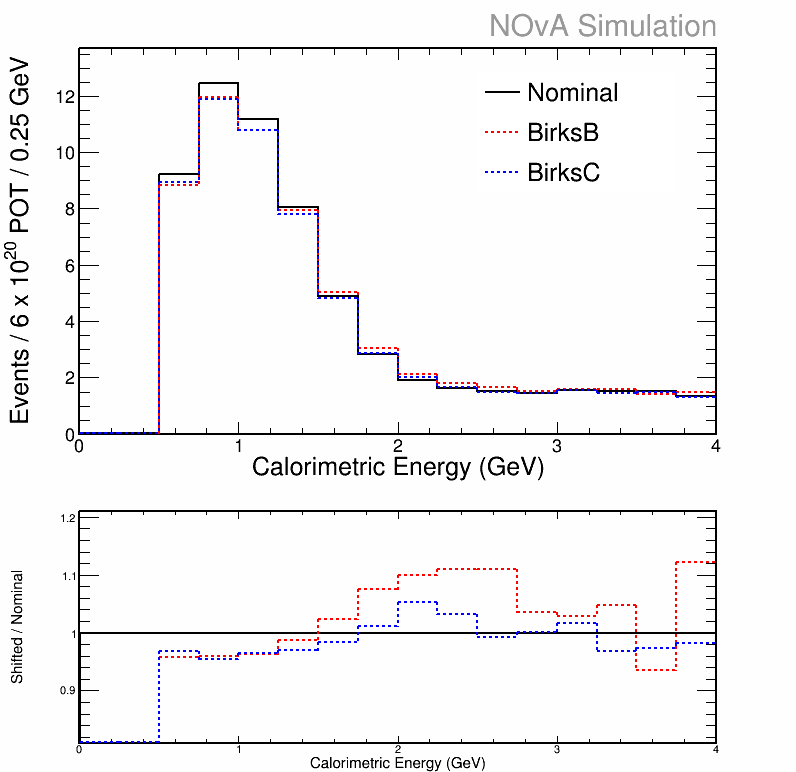
\includegraphics[width=1\linewidth]{figures/cNCEXBirksSysts.png}
  \end{subfigure}
  \begin{subfigure}{.48\textwidth}
    \centering
    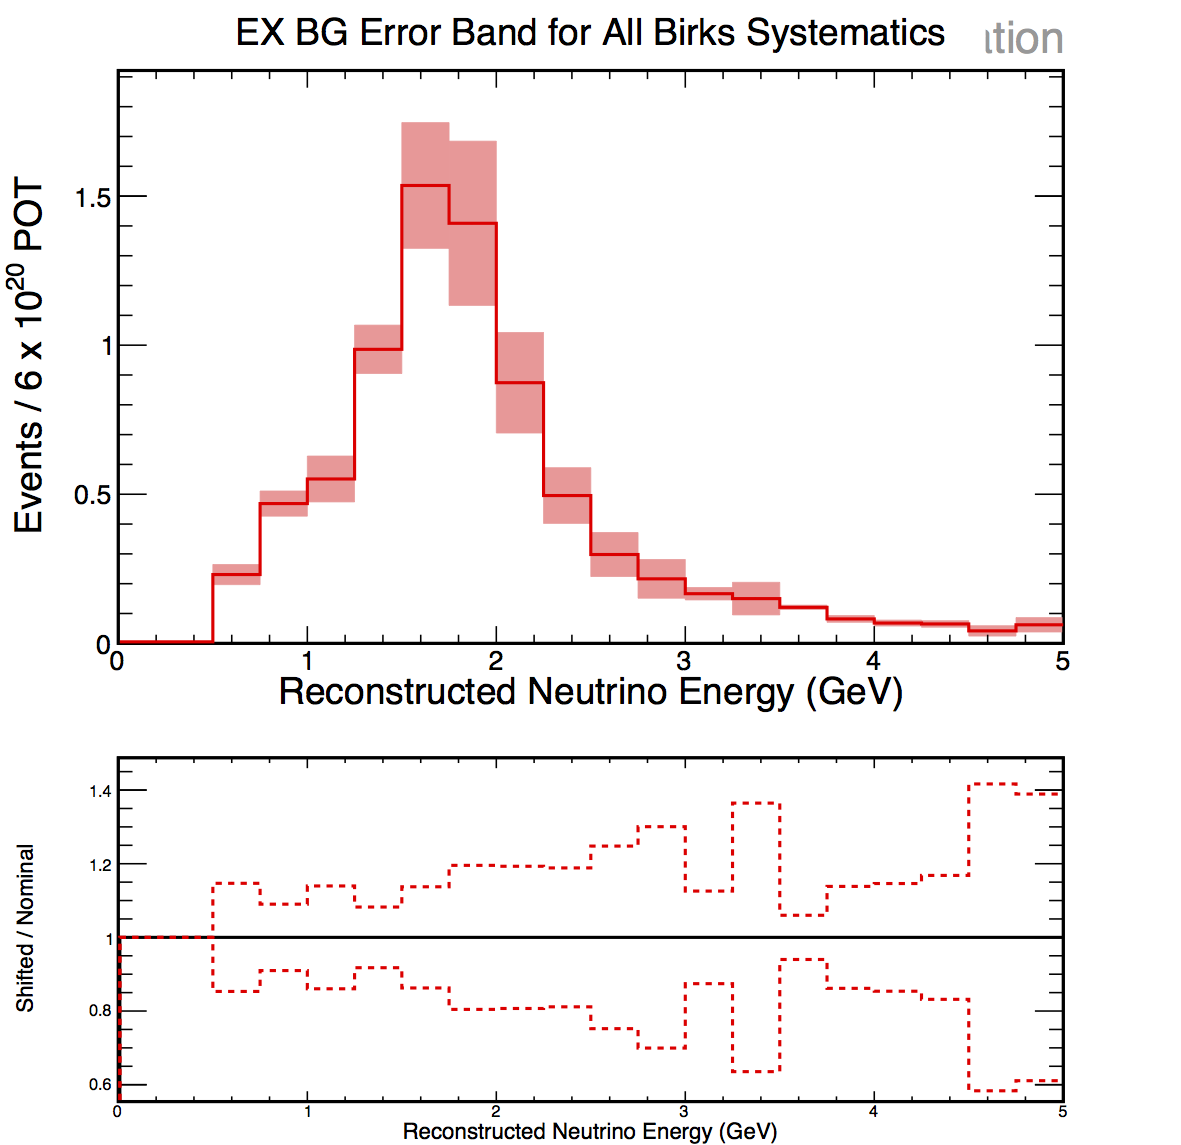
\includegraphics[width=1\linewidth]{figures/cBGEXBirksSysts.png}
  \end{subfigure}
  \caption[Birks-Chou Shifted FD Predictions]{Shifted FD predictions due to extrapolation of ND data with MC using different Birks-Chou parameter values. The NC signal spectrum is on the left; the background spectrum is on the right.}
  \label{fig:SystBirks}
\end{figure}

\subsection{Calibration}

\subsection{Detector Alignment}

\subsection{GENIE Simulation}

\subsection{Light Level Effects}

\subsection{ND Containment}

The ND does not see an effective point source of neutrinos like the FD due to its proximity to the beam source. As a result, the neutrino flux is not uniform across the detector, and so the energy spectrum of neutrinos seen by the two \nova~detectors is slightly different. To study the effect this has on the extrapolated prediction, multiple predicted FD spectra were generated using subsamples of the ND. The fiducial volume of the ND was split in half along each axis, and split into an inner and outer half (the overall containment criteria was left in tact). The extrapolation was performed using each of these `half detectors.' The error was taken as the percentage difference from the shifted prediction to the nominal. Table \ref{tab:SystFidCont} shows the results from each of these extrapolations and fig.~\ref{fig:SystsFidCont} show the shifted spectra. Like the Birks-Chou systematic, the largest overall difference was taken as the systematic error for a $TODO\%$ effect on the NC signal and a $TODO\%$ effect on the background.
\begin{table}[h]
  \begin{center}
    \caption[ND Containment Systematic Errors]{The percentage difference between the shifted and nominal predictions for the number of FD events after extrapolation using half of the fiducial volume at the ND.}
    \label{tab:SystFidCont}
    \begin{tabular}{r c c}
      \hline\hline
      ND Half & NC Difference (\%) & Background Difference (\%) \\
      \hline
      West (+X) & & \\
      East (-X) & & \\
      Top (+Y) & & \\
      Bottom (-Y) & & \\
      Front (Low Z) & & \\
      Back (High Z) & & \\
      Inner (Low $\vert$X$\vert$, $\vert$Y$\vert$) & & \\
      Outer (High $\vert$X$\vert$, $\vert$Y$\vert$) & & \\
      \hline
    \end{tabular}
  \end{center}
\end{table}

\begin{figure}[h]
  \centering
  \begin{subfigure}{.48\textwidth}
    \centering
    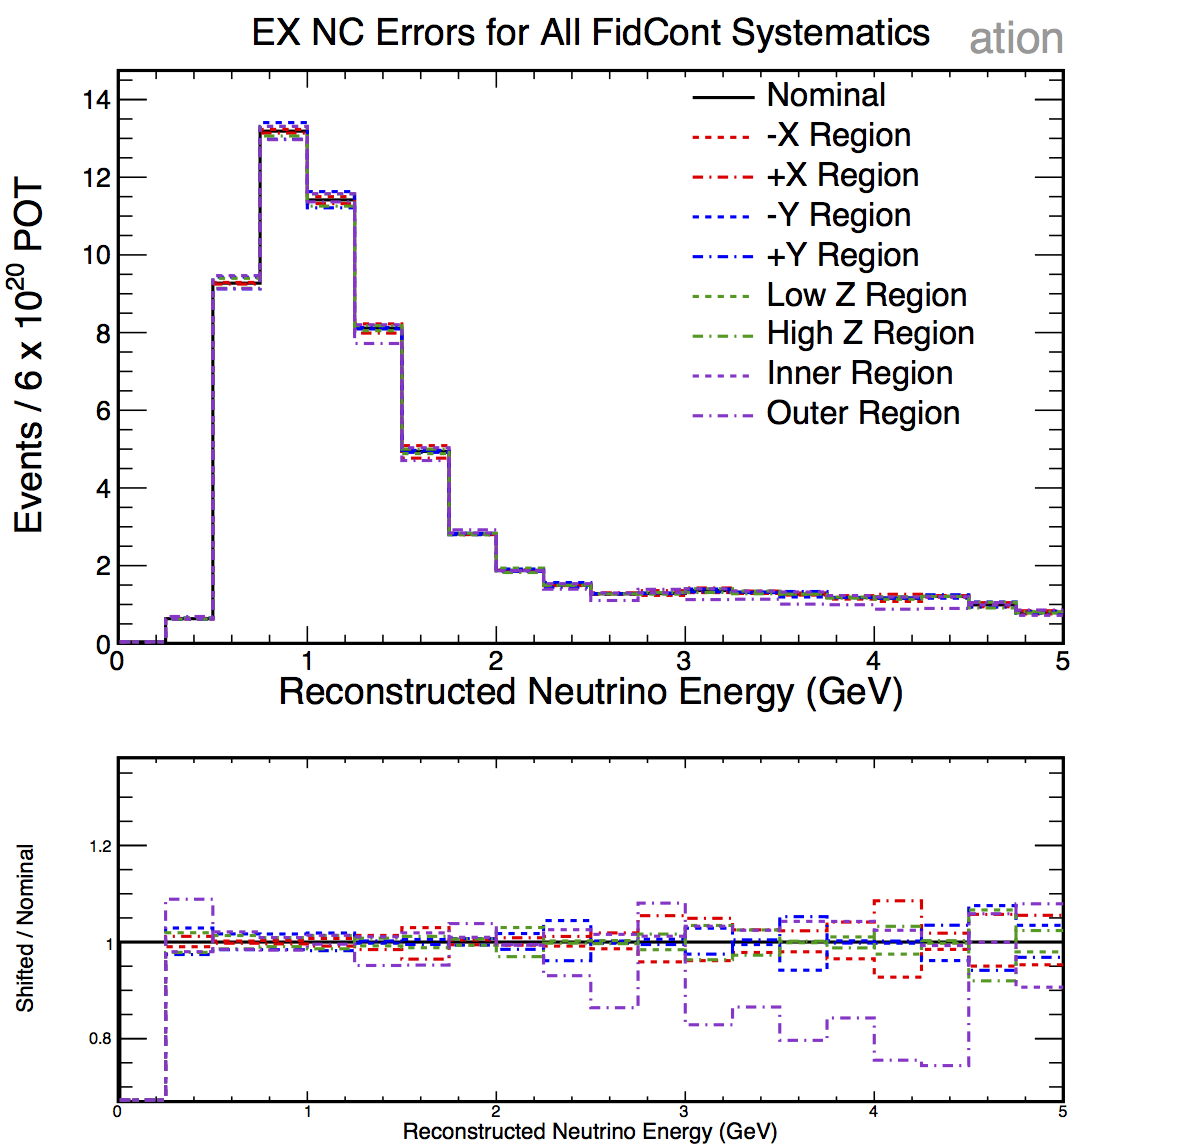
\includegraphics[width=1\linewidth]{figures/cNCEXFidContSysts.png}
  \end{subfigure}
  \begin{subfigure}{.48\textwidth}
    \centering
    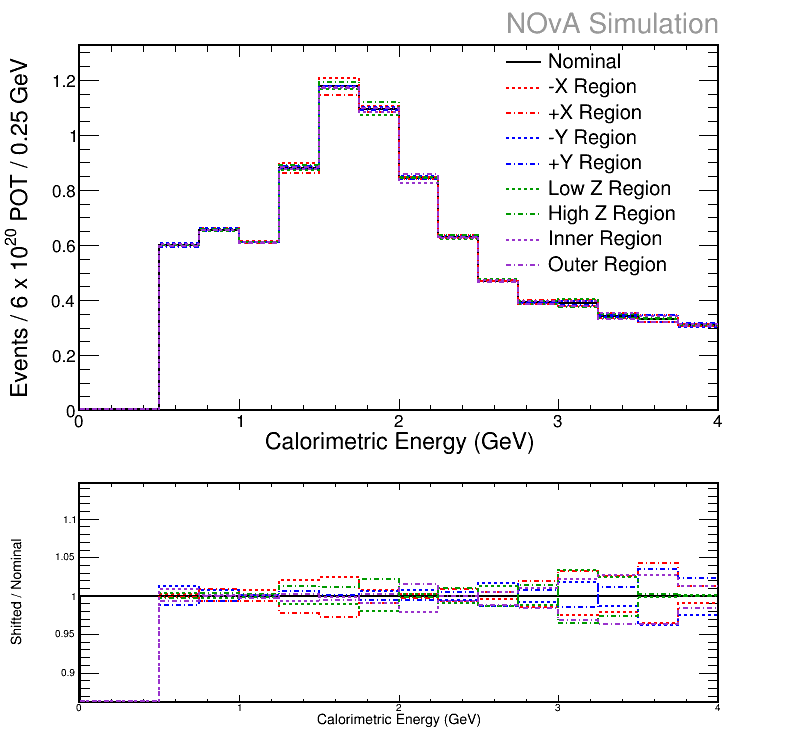
\includegraphics[width=1\linewidth]{figures/cBGEXFidContSysts.png}
  \end{subfigure}
  \caption[Shifted FD Predictions from Extrapolation of Halves of the ND]{Shifted FD predictions after extrapolation using only half of the ND fiducial volume. The NC signal spectrum is on the left; the background spectrum is on the right.}
  \label{fig:SystFidCont}
\end{figure}

\subsection{ND Rock Event Contamination}

The MC simulation does include neutrino interactions that occur in the rock that surrounds the ND. These events often leak into the detector volume, and while most of them are cut away by fiducial and containment cuts, there are some that remain. Those events that do remain cannot be reconstructed properly as their origins are outside of the detector. 

The systematic error that is incurred due to the rock event contamination was estimated by predicting the FD event spectrum from an extrapolation with rock events removed by MC truth and comparing to the nominal predicted spectrum. The events were only removed from the ND MC sample, requiring that the true neutrino vertex was inside the detector to remain. The shifted spectra are shown in Fig.~\ref{fig:SystNDRock}. This systematic amounted to an overall $TODO\%$ shift on the NC signal spectrum and a $TODO\%$ shift on the background spectrum.

\begin{figure}[h]
  \centering
  \begin{subfigure}{.48\textwidth}
    \centering
    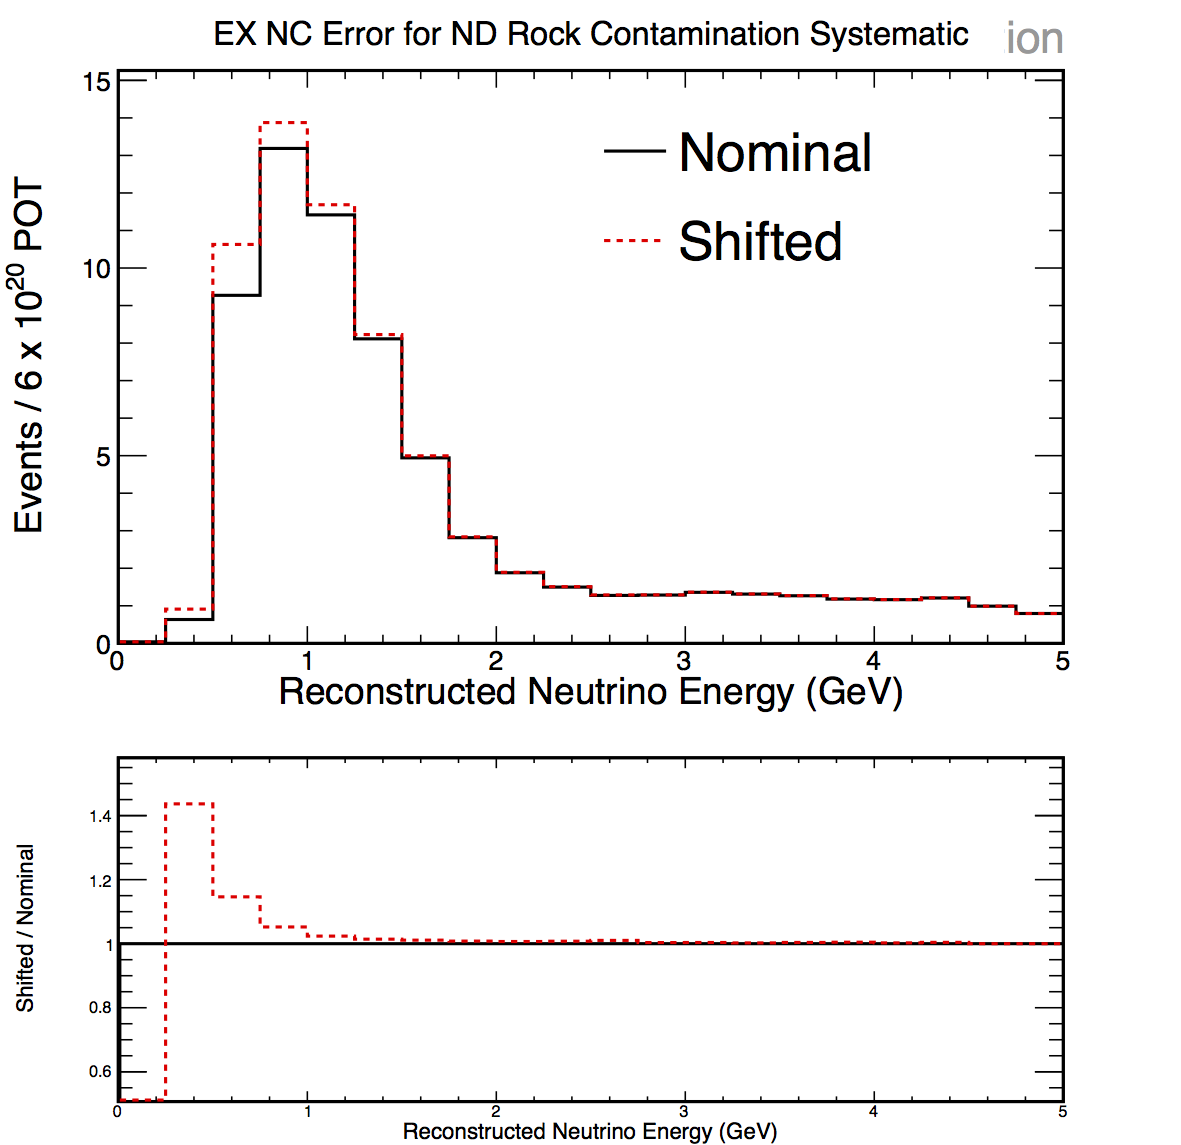
\includegraphics[width=1\linewidth]{figures/cNCEXNDRockSysts.png}
  \end{subfigure}
  \begin{subfigure}{.48\textwidth}
    \centering
    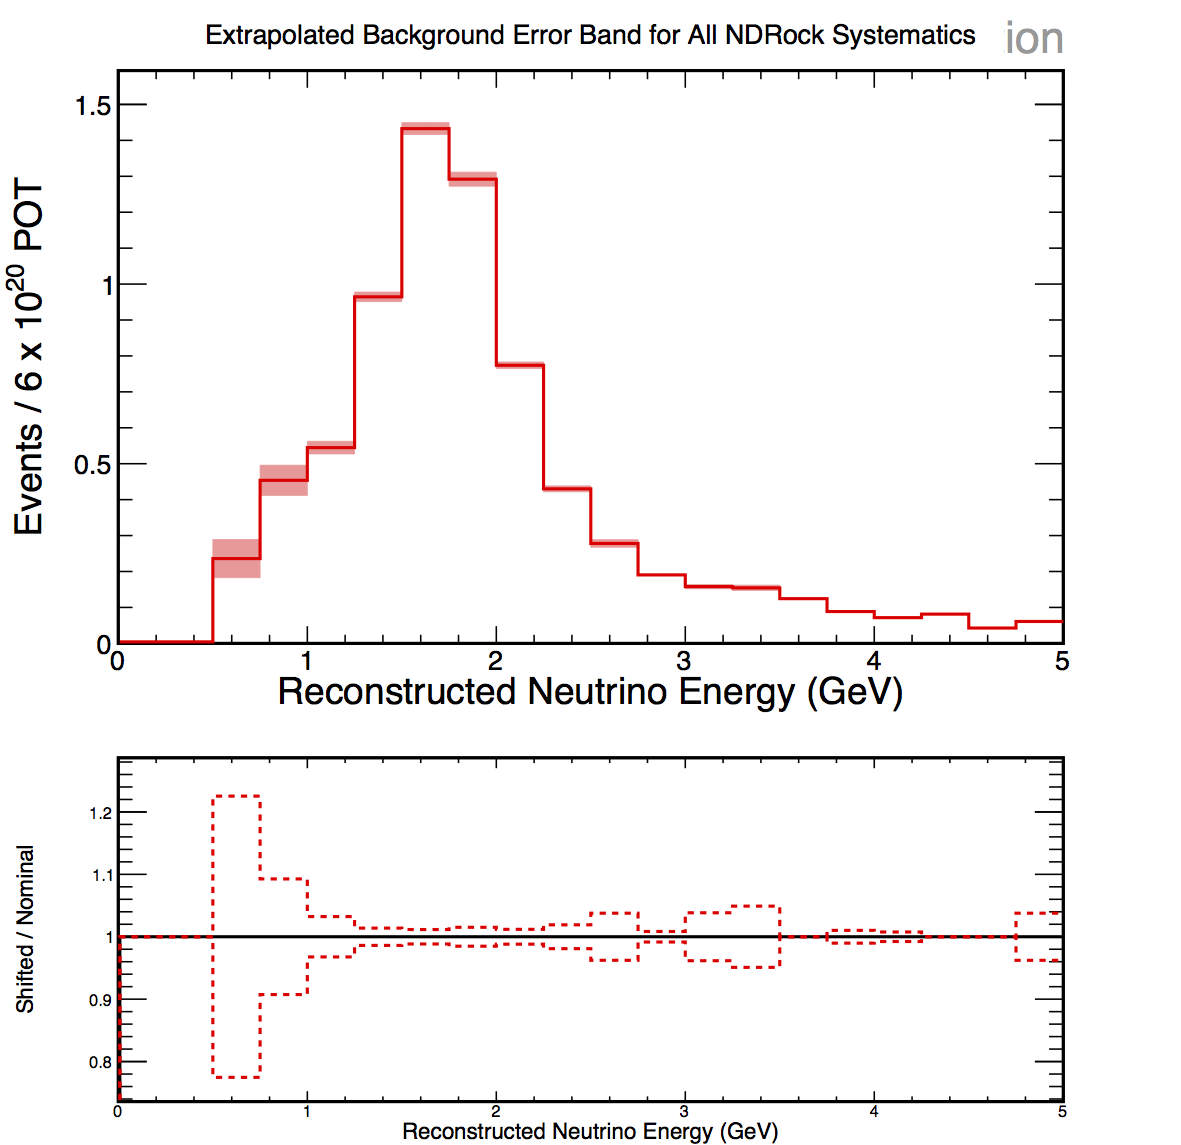
\includegraphics[width=1\linewidth]{figures/cBGEXNDRockSysts.png}
  \end{subfigure}
  \caption[ND Rock Contamination Shifted Spectra]{Shifted vs nominal spectra for the NC signal (left) and background (right). The shifted spectra are extrapolated after removal of rock events in the ND MC by truth.}
  \label{fig:SystNDRock}
\end{figure}

\subsection{ND Data/MC}

\subsection{MC Statistics}

In a perfect world, there would be enough MC statistics that this section would be unnecessary, but alas, a perfect world this is not. To estimate the systematic error due to MC statistics, the MC was split into five uniformly sized samples, and each was used to extrapolate the same set of ND data. One of the resultant predicted FD spectra was labeled as nominal, and the other four were compared to this. The bin by bin differences were taken as the error between the nominal spectrum and the `shifted' spectrum. To come up with an overall uncertainty, all of the errors were added in quadrature and the result was divided by the square root of the number of samples, or $\sqrt{4} = 2$. The result was a $TODO\%$ error on the NC signal spectrum and a $TODO\%$ error on the background spectrum.

\subsection{Overall Normalization}

Several independent effects contributed to an overall normalization systematic error. A $0.5\%$ error on the POT counting came from a small difference in the two toroids that determine the POT in a spill \cite{ref:TNBeam}. Uncertainties in the masses of the various parts of the \nova~detectors contributed another error of $0.7\%$ \cite{ref:MassError}. Finally, a study of the reconstruction efficiency between ND data and MC showed a $TODO\%$ difference \cite{ref:NDDataMCRecoEff}, which was taken directly as a contribution to the normalization error. These three effects were combined in quadrature and constituted a $TODO\%$ systematic error.

\subsection{Systematic Error Summary}

Table \ref{tab:SystSummary} shows a summary of all of the systematics, as well as an overall error. The overall error was calculated by summing the error from each row in quadrature. The final systematic error on the NC signal is $TODO\%$ and the error on the background is $TODO\%$.
\begin{table}[h]
  \begin{center}
    \caption[Systematic Error Summary]{A summary of the individual systematic errors for the NC disappearance analysis. The errors are percentage differences between the nominal and shifted predicted spectra.}
    \label{tab:SystSummary}
    \begin{tabular}{r c c}
      \hline\hline
      Systematic & NC Difference (\%) & Background Difference (\%) \\
      \hline
      Beam & & \\
      Birks-Chou & & \\
      Calibration & & \\
      Detector Alignment & & \\
      GENIE & & \\
      Light Levels & & \\
      ND Containment & & \\
      ND Rock Contamination & & \\
      ND Data/MC & & \\
      MC Statistics & & \\
      \hline
      Combined & & \\
      \hline
    \end{tabular}
  \end{center}
\end{table}

\section{Results}